\documentclass[12pt, a4paper, twoside]{article}
\usepackage{fancyhdr}
\pagestyle{fancy}
\fancyhf{}
\renewcommand{\headrulewidth}{0pt}
\addtolength{\headwidth}{\marginparsep}
\addtolength{\headwidth}{\marginparwidth}
\rhead[]{\large\textbf{EXD}}
\usepackage{fontspec}
\setmainfont{Times New Roman}
\usepackage[margin=2.5cm]{geometry}
\usepackage{amsmath,amsfonts,amsthm}
\usepackage{graphicx}
% \graphicspath{{../pdfbox/}}
%% bibliography setting nature style, footnotesize in bibliography and
%% avoiding in in articles
\usepackage[style=nature,defernumbers=true,maxnames=1,firstinits=true,uniquename=init,backend=bibtex8,arxiv=abs,mcite]{biblatex}
\bibliography{../biblio}
%\renewcommand{\bibfont}{\normalfont\footnotesize}
\renewbibmacro{in:}{%
  \ifentrytype{article}{}{%
  \printtext{\bibstring{in}\intitlepunct}}}
\DeclareFieldFormat[article]{title}{}
\AtBeginBibliography{\footnotesize}
%% to set line space in bibliography
\usepackage{setspace}
%% to add affiliation to the title
\usepackage[affil-it]{authblk}
\renewcommand\Affilfont{\itshape\small}
\setlength{\affilsep}{.2em}
%% for figure caption
\usepackage[format=plain, font=scriptsize,labelfont=bf]{caption}
%% for figure wrapping
\usepackage{wrapfig}
%% for reference in a multi col
\usepackage{multicol}
% \captionsetup[figure]{font={footnotesize, stretch=1.}, belowskip=.01pt,
%   aboveskip=0.3pt}
\captionsetup[figure]{font={footnotesize, stretch=1.}, skip=0pt}
%% titling
\makeatletter
\renewcommand{\maketitle}{\bgroup\setlength{\parindent}{0pt}
\begin{flushleft}
{\LARGE
  \textbf{\@title}}

\vspace{0.3ex}

  \@author
\end{flushleft}\egroup
}
\makeatother
\title{SOL profile and transport and relation to divertor conditions in H-Mode plasmas: a cross-machine comparison}
\author{N. Vianello$^{1}$,M. Dunne, B. Lomanowski, N. Walkden,
  M. Griener, B. Tal, W. Wolfrum, I. Cziegler, D Brida, C. Tsui,
  O. Fevrier, H. Reimerdes, C. Theiler, M. Bernert, A. Hakkola, A. Huber,
  D. Carralero$^{2, 3}$,
  V. Naulin$^{6}$,
  M. Agostini$^{1}$, J. Boedo${^5}$,
  B. Labit$^{4}$,
  H. De Oliveira$^{4}$,  the ASDEX-Upgrade Team,
  the TCV-Team, the EUROfusion MST1 Team$^{*}$}

\affil{
  $^1$Consorzio RFX, Padova,Italy,
  $^{2}$Max-Planck-Institut f{\"u}r Plasmaphysik, Garching, Germany,
  $^{3}$CIEMAT Laboratorio Nacional de Fusi{\'o}n, Madrid, Spain,
  $^{4}$EPFL-SPC, Switzerland,
  $^5$UCSD,  La Jolla, USA,
  $^{6}$DTU,  Copenhagen, Denmark,
  $^7$IPFN, Instituto Superior T{\'e}cnico, Lisboa, Portugal,
  $^{8}$CCFE, Culham, UK,
  $^9$Institute for Ion Physics and Applied Physics,
  Innsbruck,  Austria,
  $^{10}$York Plasma Institute, University of York, UK,
  $^{11}$University of Seville, Seville Spain,
  $^{12}$VTT, Espoo, Finland,
  $^{13}$Aristotle University of Thessaloniki, Greece,
  $^{14}$Jozef Stefan Institute, Ljubljana,
  $^{16}$DIFFER—Dutch Institute for Fundamental Energy Research, Netherlands,
  $^{*}$See the author list H. Meyer et al 2017 Nucl. Fusion 57 102014}
\date{\vspace{-3.5ex}}
%%% ------------------------------------------------------------
%%% BEGIN DOCUMENT
%%% ------------------------------------------------------------
\begin{document}
\maketitle
\vspace{-1.2em}
{\it \small Corresponding Author:} {nicola.vianello@igi.cnr.it}

Plasma Exhaust and Plasma Wall Interaction (PWI) are subjects of intense studies
in the context of fusion energy research for the understanding of the amount of heat
loads, tritium retention, and the lifetime of different Plasma Facing
Components. On this context in order to ensure reliability of
predictive edge modeling for future devices, it is mandatory to
determine the transport properties of the Scrape Off Layer (SOL) in
condition close to the operational point foreseen for ITER and future
devices. From the ITER divertor perspective, to
keep the power fluxes densities acceptable for target material,
high neutral pressure and partial detachment are needed to
ensure maximum tolerable loads based on avoidance of W
recrystallization \cite{pitts:2019}. Thus experimental investigation
of SOL transport needs to be extended also to these operational regimes.
The SOL properties results from a competition between sources and losses parallel and
perpendicular to the magnetic field: it is strongly dominated by
the presence of turbulent filaments, which strongly contribute to
particle and energy losses both in L- and H-mode regimes.
In present experiments the regimes matching ITER divertor operational point are obtained
with high gas throughput leading to high density regimes. In L-Mode
these operational conditions are associated to the appearance of a
\emph{density shoulder}
i.e. progressive flattening of the density
scrape off layer profile at high density
\cite{Asakura:1997is,LaBombard:2001ks,Rudakov:2005ic,
  Carralero:2015gu}. It has been proved that density shoulder appear
starting from high-recycling regimes and become broader after target
density rollover \cite{vianello:nf2019}, even
though differences have been observed depending on divertor geometry
\cite{Wynn:2018gp}, or if high recycling condition are achieved
through impurity seeding rather than high fuelling
\cite{Wynn:2018gp,Kuang:2019248}. The density shoulder is actually accompained by
an increase of the filamentary activity
\cite{Carralero:2015gu,Vianello:2017ku,Kuang:2019248}, together with an increase of
their associated convective transport \cite{Carralero:2017gb},
Preliminary investigations suggested that similar inter-ELM SOL
density profile broadening is observed in H-mode as well
\cite{Muller:2015jt,Carralero:2017gb,vianello:nf2019}, with a stronger
dependence on the neutral pressure \cite{vianello:nf2019}. Furthermore
in case of highly dissipative divertor with high gas throughput the
pedestal profile modification move the plasma towards a small-ELM
regime \cite{labit:nf2019,Harrer:2018jn} wheare a clear increase of
the SOL density decay length is observed.

Despite the
large experimental effort, a comprehensive understanding
of the mechanism leading to an H-mode shoulder formation is presently
lacking and this motivated a joint experimental within the european tokamaks.
The present contribution will indeed report results obtained in a
coordinated effort within 3 different devices, JET, ASDEX-Upgrade (AUG) and
TCV focusing on the SOL profile evolution in different divertor recycling
states, correlating the observed profile modification with different turbulent SOL
plasma transport.
\begin{wrapfigure}{l}{100mm}
\centering
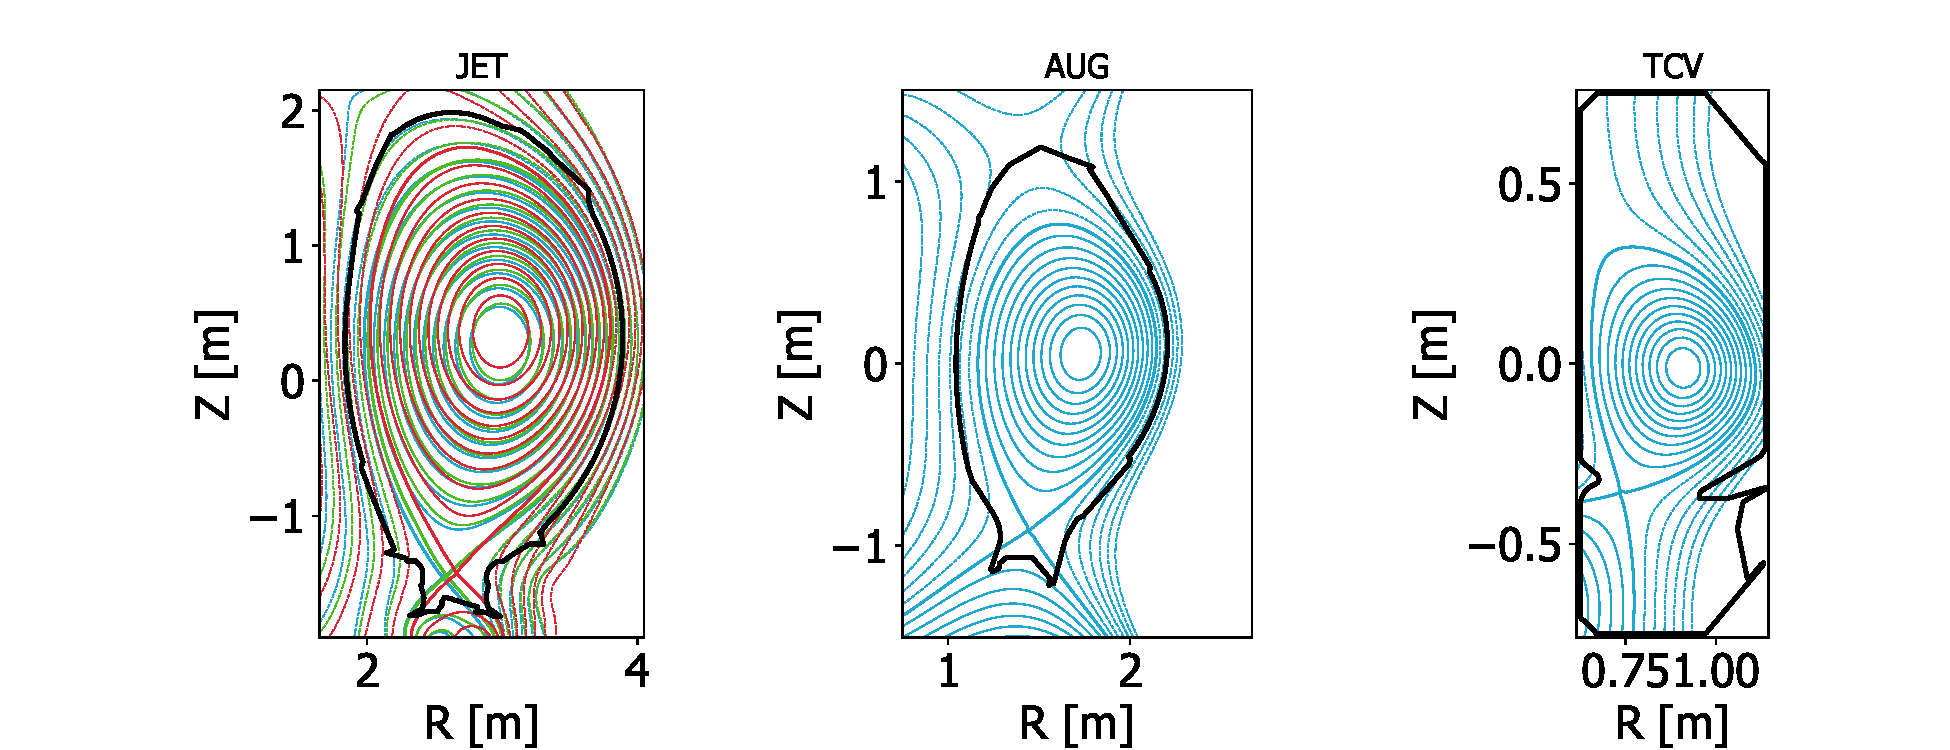
\includegraphics[width=100mm]{../pdfbox/AllEquilibria.pdf}
\caption{Plasma shapes investigated in all the three devices. For JET
  the 3 different configuration are shown as well}
\vspace{-2.6ex}
\label{fig:fig1}
\end{wrapfigure}
\ref{fig:fig1} shows the typical plasma shapes used in the present
investigations.
In JET, 2MA/2.3T low-$\delta$ plasma with 16 MW of
applied NBI power were analyzed, where plasma divertor shapes
were investigated in horizontal or vertical targets in order to take
advantages of the different neutral compression achieved
\cite{Tamain:2015cx}. Plasma fuelling in the different divertor
configurationx has been varied to explore different recycling states
determined by spectroscopic measurement combined with langmuir probes
embedded on the tiles. On AUG 0.8MA/2.1T scenarios were investigated
where different power levels (from 3 to 17 MW) and different fuelling
schemes were used in order to explore a wide range of divertor
parameters and recycling state. Finally on TCV high-$\delta$ low current (0.18 MA)
discharges were investigated with an additional 1 MW of NBI heating
where different fueling levels and fueling scheme (main chamber or
divertor fuelling) were used. In all the devices if we determine
inter-ELM profiles at different recycling states explored through
fueling changes, we observe a clear SOL profile broadening as shown in
figure \ref{fig:fig2}.


\begingroup
\setstretch{0.8}
{\footnotesize\textbf{Acknowledgment}\\
This work has been carried out within the framework of the EUROfusion Consortium and has received funding from the Euratom
research and training programme 2014-2018 under grant agreement No 633053. The views and opinions expressed herein do not
necessarily reflect those of the European Commission.}
\begin{multicols}{2}
\setlength\bibitemsep{0pt}
\printbibliography[heading=none]
\end{multicols}
\endgroup

\end{document}

% \begin{wrapfigure}{l}{67mm}
% \centering
% \includegraphics[width=67mm]{../pdfbox/EfoldBlobAllColor.pdf}
% \caption{Top: Density decay length as a function of blob size
%   at three level of currents at constant B$_t$ in
%   AUG. Bottom: same for TCV}
% \vspace{-2.6ex}
% \label{fig:fig1}
% \end{wrapfigure}

% \begin{wrapfigure}{l}{96mm}
% \centering
% \includegraphics[width=96mm]{/Users/vianello/Desktop/Topic-21/Experiments/AUG/analysis/pdfbox/UpstreamDivertorProfiles34276_34278_34281}
% \caption{ Shots
%   \# 34276 and shot \# 34278 have the same fueling and seeding levels,
%   but the shots have been operated respectively without and with
%   the cryopump. Additional fueling and seeding have been added to Shot
%   \#34281 where cryopump was in operations. The top
%   panel show the time traces of edge density. The second rows show the
% upstream profiles normalized to the value at the separatrix for the
% three shots in 3 time instants indicated in the top panel with
% different colors. The third rows report the target profiles at
% the same instants whereas the last rows show the value of divertor
% normalized collisionality $\Lambda_{div}$ as defined \cite{Carralero:2015gu}}
% \vspace{-2ex}
% \label{fig:fig2}
% \end{wrapfigure}
